\documentclass{ieeeaccess}
%\usepackage{cite}
\usepackage{amsmath,amssymb,amsfonts}
\usepackage[square, comma, sort, numbers]{natbib}
\usepackage{algorithmic}
\usepackage{graphicx}
\usepackage{textcomp}
\usepackage[hyphens]{url}
\usepackage{hyperref}
\def\BibTeX{{\rm B\kern-.05em{\sc i\kern-.025em b}\kern-.08em
    T\kern-.1667em\lower.7ex\hbox{E}\kern-.125emX}}

\begin{document}
\bstctlcite{BSTcontrol}

\history{Date of publication xxxx 00, 0000, date of current version xxxx 00, 0000.}
\doi{10.1109/ACCESS.2017.DOI}

%Lucas Marques da Cunha: https://orcid.org/0000-0003-1555-2505
%Patrick Terrematte https://orcid.org/0000-0002-0385-0030 
%Tayná da Silva Fiúza: https://orcid.org/0000-0002-6455-7698 
%Vandeclécio L. da Silva https://orcid.org/0000-0002-9551-4076 
%José Eduardo Kroll https://orcid.org/0000-0002-7657-9536 

\title{dbPepVar: a novel cancer proteogenomics database}
\author{\uppercase{Lucas Marques da Cunha}\authorrefmark{1,2}, \uppercase{Patrick Terrematte}\authorrefmark{1,3},
\uppercase{Tayná da Silva Fiúza}\authorrefmark{1},
\uppercase{Vandeclécio L. daSilva}\authorrefmark{1},
\uppercase{José Eduardo Kroll}\authorrefmark{1}, \uppercase{Sandro José de Souza}\authorrefmark{1,4}, \uppercase{Gustavo Antônio de Souza}\authorrefmark{1,5}}

\address[1]{Bioinformatics Multidisciplinary Environment - BioME, Federal University of Rio Grande do Norte - UFRN, Brazil}
\address[2]{Federal University of Rondonia - UNIR, Brazil}
\address[3]{Metropolis Digital Institute, UFRN, Brazil}
\address[4]{Brain Institute, UFRN, Brazil}
\address[5]{Department of Biochemistry, UFRN, Brazil}

\tfootnote{``This work was supported in part by the grants 23038.004629/2014-19 to GAS from the Coordenação de Aperfeiçoamento de Pessoal do Ensino Superior. GAS was also supported by grants 406630/2016-0 and 304422/2017-7 from Conselho Nacional de Desenvolvimento Científico e Tecnológico (CNPq). LMC, VLS, JEK, TSF were funded by CAPES –  Coordination for the Improvement of Higher Education Personnel formation programs. This publication was supported by the Fund of the Federal University of Rio Grande do Norte.''}

\markboth
{Cunha \headeretal: dbPepVar: a novel cancer proteogenomics database}
{Cunha \headeretal: dbPepVar: a novel cancer proteogenomics database}

\corresp{Corresponding author: Lucas Marques da Cunha (e-mail:  lucas.marques@unir.br, ORCID: \url{https://orcid.org/0000-0003-1555-2505}).}


\begin{abstract}

Cancers arise from the acquisition of DNA mutations, such as substitutions, deletions, amplifications, and rearrangements. Understanding the distribution and correlation of such mutations in cancer may aid the characterization of the disease and subsequent identification of biomarkers for diagnosis and treatment. The proteogenomics database (dbPepVar) created here combines genetic variation information from dbSNP with protein sequences from NCBI's RefSeq. Public mass spectrometry datasets (Ovarian, Colorectal, Breast, and Prostate) were used to perform a pan-cancer analysis, allowing the identification of unique genetic variations. As a result, 3,726 variant peptides were identified in samples from patients with ovarian cancer,  2,543 in prostate, 2,661 in breast and 2,411 in  colon-rectal cancer patients. Data resulting from the proteogenomics approach employed and connected to other biological databases is now available in an intuitive and dynamic web portal where novice users can explore general aspects of the dataset in graph or table format, or dive in to filter the data with click and select options or using more advanced queries with regex. All data can be downloaded in csv or pdf format. In perspective, the web portal developed may direct studies to identify new therapeutic targets for different cancers, and one can also use our database for characterization of variants in samples of unknown genetic background, such as archived samples.
\end{abstract}

\begin{keywords}
Cancer proteomics, Genetic variation, Proteogenomic Database.
%Enter key words or phrases in alphabetical order, separated by commas. For a list of suggested keywords, send a blank e-mail to keywords@ieee.org or visit \underline {http://www.ieee.org/organizations/pubs/ani_prod/keywrd98.txt}
\end{keywords}

\titlepgskip=-15pt

\maketitle

\section{Introduction}
\label{sec:introduction}
\PARstart{M}{ass} spectrometry (MS) based proteomics has become the primary method for comprehensive protein detection and characterization. Peptide identification is often based on challenging experimental peptide MS spectra against theoretical peptide data created from a protein sequences database such as RefSeq, Uniprot, or Gencode \cite{Sheynkman2016-fo}. Those databases for protein identification do not take into consideration genetic variations in populations. This genetic variability gives individuals unique phenotypic characteristics, vulnerability to diseases, and profiles of responses to drugs. Variations in genomes are mainly caused by single nucleotide polymorphism (SNPs), insertions, deletions, and changes in the number of copies (CNVs). Some might affect protein-coding sequences, producing not only a single amino acid change but also changing the reading frame, originating abnormal sequences, or removing whole portions of the protein through a premature termination codon insertion \cite{Vegvari2016-qm, Renuse2011-wl}. Thus, peptides whose exact sequences are not found in the databases remain unidentified. Some missing sequences might have a central biological role in non-annotated protein-coding regions, specific variations of individuals, or for a specific disease mutation. So the characterization of those new proteoforms is essential for understanding human biology \cite{Sheynkman2016-fo}. To grasp full information on protein variations, it is usual to apply proteogenomics methods, a field on the intersection between genomics and proteomics.

Proteogenomics assists in the identification of new coding variants by searching the MS/MS spectra against a database of customized proteins. The protein sequences in these databases are constructed using genomic and transcriptomic information that is absent in conventional protein databases. The approach improves the annotation at the protein level, refines gene models, characterizes protein isoforms, restricts the location of the translation start and end sites, identifies splice sites, and alternative forms of splicing \cite{Menschaert2017-ov, Ruggles2017-ez, Nesvizhskii2014-ej, Castellana2010-ro}. In precision medicine, proteogenomics is widely used as an alternative to detect mutations in different cancers to find new biomarkers for tumors, analyze differences in levels of gene expression, compare variants to patient survival and support the development of new drugs \cite{Woo2014-tk,Zhang2014-rb}. 

The customization of such proteogenomics databases is achieved according to the research goal. For instance, one of the widely used alternatives is the creation of a database generated from the translation of the six reading frames. However, this approach is limited because of the increase in the database search space and the fail to capture peptides present at the junction between exons \cite{Nesvizhskii2014-ej, Renuse2011-wl}. Other approaches develop a database incorporating mutations into populations of selected reference sequences and report the variant sequence with a special character \cite{Schandorff2007-ro}. The variations can be downloaded from the NCBI's dbSNP database and supplemented with mutations of known diseases from the public database such as \textit{Online Mendelian Inheritance in Man} (\url{https://www.ncbi.nlm.nih.gov/omim}) or \textit{Protein Mutant Database} (\url{https://www.rcsb.org}). In another case, a database of tryptic peptides was created from information found in NCBI's dbSNP \cite{Bunger2007-yo} by adding to the database only the mutated tryptic peptides and the corresponding reference peptides, an approach distinct from \cite{Schandorff2007-ro}, which maintained the complete reference sequence. Regarding the variations, only nonsynonymous mutations and indels (insertions and deletions) that do not generate frameshift were incorporated. Applications of such databases include the investigation of neglected tropical diseases \cite{Pawar2014-gl}, Alzheimer's disease \cite{Da_Silva2021-cq}, and other complex conditions, like cancer. 

Cancer, as a complex disease, arises from combinations of mutations on the same cells over time \cite{Hahn2002-bo}, \cite{Whitworth2016-lr}, triggered by external and endogenous factors \cite{Eccles2016-yq,Adi-Kusumo2016-cd}. Distinct cancer types present different combinations of mutations \cite{Hahn2002-bo}, \cite{Whitworth2016-lr}. Mutations may alter the efficiency of molecules by hindering their stability and activity. In cancer etiology, such mutations can occur in specific genes, called proto-oncogenes, which are initially inactive in normal cells. After being activated, proto-oncogenes become oncogenes, responsible for transforming normal cells into cancer cells. Current techniques seek to identify these changes and determine the impact generated on gene products such as RNAs and proteins, which play a major role in the cellular functions of an organism's processes. In cancer, aberrant proteins stimulate initiation, progression, and response to treatment. The abundances of protein and mRNA molecules are partially correlated and determining how the flow of information culminates in proteomic changes in tumors is a major under-explored issue in cancer biology \cite{Alfaro2014-dg}. An exclusive set of alterations can define a subtype profile in a cancer type \cite{Redei2008,Hahn2002-bo}. The SNPs play a fundamental role in distinct responses to the treatment of cancer patients, and also might characterize the risk of low survival outcomes \cite{Hahn2002-bo}, \cite{Whitworth2016-lr}, \cite{Deng2017-kq}. The presence of mutations in coding regions might affect cellular signaling pathways, as well as the levels of oncogenic and tumor suppressor proteins \cite{Deng2017-kq}. 

Researchers have been developing solutions for better integrating variant discovery into proteomics studies. The Cancer Proteome Variation Database (CanProVar) integrates public data information on protein variations, provides access to known variations in proteins related to cancer types, and evaluates the impact of these variations on their functional characteristics \cite{Li2010-px,Zhang2017-yz}. The CanProVar provides a base rich in genetic variations related to different cancer, incorporating missense, nonsense mutations, and single-base insertions and deletions derived from specific cancer bases, such as TCGA, HPI, COSMIC, and OMIM. Although there is a great diversity of variations incorporated, the base does not include untranslated region (UTR) mutations. The database Swiss-CanSAAVs was developed using the unique variant sequences of the \textit{Humsavar} database, which contains only missense mutations, and integrating the MS-CanProVar database with the canonical protein database UniProtKB/Swiss-Prot  \cite{Song2014-bn}. For each single amino acid variation, an independent tryptic peptide with two missing cleavage sites around the central variation site was extracted from the protein sequences, and an identifier prefixed with SAAV was adopted to differentiate from the canonical protein sequence. For instance, the database Swiss-CanSAAVs was used to identify profiles of amino acid variants of subpopulations in the breast cancer cell line MCF-7 \cite{Tan2017-ut}, identifying protein sequences \cite{Song2014-bn}. The dbSAP database presents a set of variants derived from eight different SNP databases and was used to characterize mutations in various types of cancer \cite{Cao2017-pv}. Similar work has been done by \cite{Alfaro2017-vp} using a combination of publicly available population variants (dbSNP and UniProt) and somatic variations in cancer (COSMIC), along with sample-specific genomic and transcriptomic data to examine the variation in the proteome within and across 59 cancer cell lines. 

Those databases kept variant and reference sequences within a single file. Most peptide search engines use algorithms based on statistical analysis. Such an algorithm might not assign a mutated peptide correctly because of minimal differences in each score value between the variant and reference sequences \cite{Lane2005-nj}. Furthermore, the approaches described above are limited to some mutations, allowing only databases with missense mutations and small insertions/deletions mutations. The mutations with the most significant impact on the sequence and protein function, such as frameshifts, variation of start translation, and loss of stop codon also are not included \cite{Choi2012-jh,Hu2012-wm,Banfai2017-ql}. 

In this article, we present a variant database called dbPepVar, which contains mutated peptides combining information from the dbSNP and RefSeq. Compared to other approaches as those described above, our database reports a greater diversity of variants, including missense, nonsense mutations, loss of termination codon, insertions, deletions (of any size), frameshifts, and mutations that alter the translational starting site. Furthermore, for each protein, only the variant tryptic peptides derived from enzymatic cleavage (i.e., trypsin) are stored, following the criteria of size, allelic frequency, and affected regions of the protein. In our approach, MS data is submitted to the dbPepVar variant and a reference database separately. The outputs are compared and filtered by the scores for each peptide identification. Using public MS data from four types of cancer, a majority of SNPs were identified, but cancer-shared mutations were also present in a lower amount.

\section{MATERIALS AND METHODS}

\subsection{Data source}

To generate the dbPepVar variant database, we used the protein RefSeq data (\url{https://ftp.ncbi.nlm.nih.gov/refseq/H_sapiens/mRNA_Prot/}) and the dbSNP (\url{https://ftp.ncbi.nlm.nih.gov/snp/}), both available on the NCBI portal. To carry out identifying variants in different types of cancer, we used experimental mass spectrometry data derived from samples from four studies: ovarian cancer \cite{Coscia2016-zq}, prostate cancer \cite{Iglesias-Gato2016-cb}, colorectal cancer \cite{Zhang2014-rb}, and breast cancer \cite{Tyanova2016-sz}. All MS raw data is available at the ProteomeXchange repository (\url{https://www.proteomexchange.org}).

\subsection{Data preprocessing}

Initially, the dbSNP data were preprocessed to remove redundancies, inconsistencies, and incompleteness. The mutations of Leu to Ile or Ile to Leu were discarded since both amino acids have the same molecular mass and are not distinguished by mass spectrometry. We also removed mutations leading to alternative splicing and synonymous mutations. At the end of this process, three new files were generated containing information about the SNP, indel in-frame, and frameshift mutations. From the file containing the SNPs, four new files were generated, separated by the categories of stop-loss, untranslated region Variation (UTR variation), rare SNPs (Minor Allele Frequency $<$5\%), and common SNPs (Minor Allele Frequency $\geq$ 5\%) \cite{International_HapMap_3_Consortium2010-eo}. For each type of mutation, Perl scripts were implemented to create the new proteoforms according to each mutation type described. All files processed from dbSNP contain the RefSeq identifier of the protein (NP Accession), the reference amino acid, the mutated amino acid, the position of the mutation, and the SNP identifier (RefSNPs, rs).

\subsection{Creation of the proteogenomics base}

The first step in creating the variant database is to generate a multi-fasta file containing the proteoforms according to the dbSNP information and then extract the variant tryptic peptides. To generate the multi-fasta file, six scripts were developed in the Perl language, referring to each type of mutation: rare SNPs, common SNPs, indel in-frame, indel frameshift, stop-loss, and UTR variation. The multi-fasta files were used as input to a second script that performs the search for the tryptic peptides variant of each proteoform. The third script generates a file in the multi-fasta format, concatenating all the variant tryptic peptides for each protein.
In this process, we discard variant peptides that had less than or equal to 7 amino acid residues and that were greater than or equal to 35 residues \cite{Fricker2015-eh}. Due to post-translational processes, a protein can undergo internal cleavages, such as the removal of the initial methionine (Met), to generate a mature product of smaller size \cite{Strachan2002-an}. Therefore, for any N-terminal tryptic peptides, we report a duplicate with and without the initial Met. Similarly, in cases where the protein contains a C-terminal peptide with over one mutation or had more than one nonsense mutation, we generate a new entry in the fasta file for any additional peptide variation. Otherwise, the identification software could interpret them as a single peptide, as the C-terminal peptide could lack a tryptic cleavage site (Arg or Lys). For the peptides in which the mutation has removed or added a cleavage site, we verify whether the number of residues remained within the range established in our approach.

The SNPs detected from a particular protein-coding region by NGS technologies in a tumor tissue sample are possibly derived from heterogeneous cells \cite{CHOONG2020}. Furthermore, non-random genetic variations tend to occur together, as haplotypes inherited from a single parent are linked on the same chromosome \cite{CHOONG2020}. Therefore, peptides that showed more than one mutation were reported according to the number of possible combinations. This criterion is made only for peptides SNP-type mutations with a common allelic frequency (Minor Allele Frequency $\geq$ 5\%) to reduce computational complexity. Using this criterion only for common mutations also allows us to reduce the search space and to avoid undesirable combinations with other types of mutations. The number of combinations that a peptide can present is according to the formula $2^n - 1$, where n is the number of mutations. For instance, for a peptide that has 12 mutations, the number of combinations will be $2^{12} - 1$ = 4,095 peptides that will be generated. This process is described in Fig. S3.

For frameshift and stop-loss mutations, we developed a script that performs the mutation in the mRNA and translates it to the respective protein. After this process, we report the variant peptide sequence that starts at the point where the mutation occurred. Missense mutation can also alter the mRNA's untranslated region (UTR variation) by replacing the base in the initial codon. In this way, the translation machinery scans up to the next initial ATG nucleotide codon triplet \cite{Hinnebusch2016-ta}. In this case, we report the tryptic peptide corresponding to the new start of the translation of the protein.

We also implemented scripts to extract information such as the protein identifier (NP accession), the SNP identifier (RefSNP, rs), the position of the mutation in the sequence protein, the reference tryptic peptide, and the mutated peptide. This information was useful for missed cleavage analysis and for classifying the peptides according to their mutation type.

\subsection{MS identification and analysis of the identified peptides}

The LC-MS data in RAW format was analyzed by MaxQuant (version 1.6.14), using previously described parameters \cite{Machado2019-sj}. The peptide identification process was carried out using a two-stage strategy, where the MS data were sought first using the human proteome Refseq and, later, were searched using the personalized dbPepVar database. After each stage, the ``evidence.txt'' files are generated regarding the identification of the peptides according to the search base used. The evidence file combines all information about the identified peptide spectrum matches (PSM) and is usually the only file needed for processing the results.

Initially, we remove false positives and contaminants identifications. For data provided from the Super-SILAC quantification protocol (Breast and Prostate cancer), peptides with an Intensity value of L = 0 (i.e., only identified in the reference Super-SILAC cells) are removed, as it shows that the peptide was not detected in the non-reference sample. The next step is to analyze the quality of the peptide scores and select those that have the best value. All peptides identified in dbPepVar with a score lower than 50 were removed as they indicate low-quality identification.

We compared the two evidence files obtained from the two RefSeq and dbPepVar databases to check if there are two different sequences identified to the same MS spectrum. For this, the fields of the evidence file Raw File and MS/MS Scan Number are used to generate a unique identifier of the PSM. A Perl script was implemented to check and add to a file the peptides that were identified on both databases. In cases of a conflict, the script selects the variant peptide only when its score is 20\% higher than the score of the RefSeq sequence identified for the same spectrum.

During the proteolytic digestion process, the enzyme can fail to cleave in one or more tryptic sites. Therefore missed cleavages are often considered  during peptide identification. In the evidence file obtained from dbPepVar, we verify whether the peptides that showed missed cleavages were possible false positives. We considered false-positive variant tryptic peptides with missed cleavage whose location contradicted the actual position in the original protein. This occurs because the way our database is created, mutated peptides are concatenated even though they are not necessarily neighbouring peptides in the reference protein. For this analysis, we used the field Missed cleavages in the evidence  table, where values greater than 0 indicate the presence of a missed cleavage. The registration file was used to check the position of the peptide in the source protein. In this filtering process, we also discard the variant peptides that were also present in the RefSeq base. Moreover, for mutations of the UTR variation type, we discard peptides that had a cleavage site before methionine, avoiding an erroneous identification of an enzymatic cleavage as a false new start of translation.
We then classify the variant peptides according to the type of mutation. The information was obtained from the log files generated in the creation of the dbPepVar database. As an output, we extract two new fields to the evidence files regarding the type of mutation and the dbSNP code. To visualize the mass spectra of the identified peptides, we used a tool called Proteogenomics Viewer \cite{Kroll2017-ab}. It is a web tool that collects the identification of peptides by mass spectrometry, indexes a sequence of genetic structure, attributes the use of the exon, and relates to isoforms of proteins. Thus, to suit the data to the tool, we generate a protein sequence base, replacing the reference sequence or peptides used by the MS for each type of cancer. In cases where different variant peptides are used for the same protein and position, a new sequence is generated for each variation.

\section{RESULTS}

\subsection{Building dbPepVar and identification of variant peptides by MS}

The dbSNP data was processed by selecting and categorizing types of mutations according to genomic coding  region and impact on the protein sequence. Mutations where there was an uncertainty of the actual biological event, e.g.: when mutations were represented by a question-mark, were discarded. A total of 10,490,264 SNPs were selected from dbSNP, 10,417,131 with minor allele frequency (MAF) $<$ 5\% and 73,133 with MAF $\geq$ 5\% \cite{International_HapMap_3_Consortium2010-eo}. The other selected types of mutations were indels (194,056), stop-loss (10,753), translational start sites (24,195), and frameshifts (367,348). In the end, 11,086,616 mutations were considered. These data were used as input for the construction phase of the dbPepVar database, generating a total of 7,747,637 tryptic peptides. For comparison, this database is approximately seven times larger than the Refseq (1,174,168 tryptic peptides). Fig. 1 shows the workflow used to create the dbPepVar database. Fig. S1 shows the process used to report the variant peptides. As additional data to dbPepVar, a file was generated containing information about the mutated peptide, such as its SNP identifier, the location of the mutation in the protein, and the sequence of the reference peptide (see Fig. S2). This information allows the validation of genomic variants at the proteomic level, the location of the type of mutation that affects the peptide, the association of the variant peptide with the corresponding SNP, and the analysis of heterozygosity, through the screening of samples that show the identification of mutated peptides and variants. 

\begin{figure*}[htpb]%
\centering
%{\color{black!20}\rule{213pt}{37pt}}
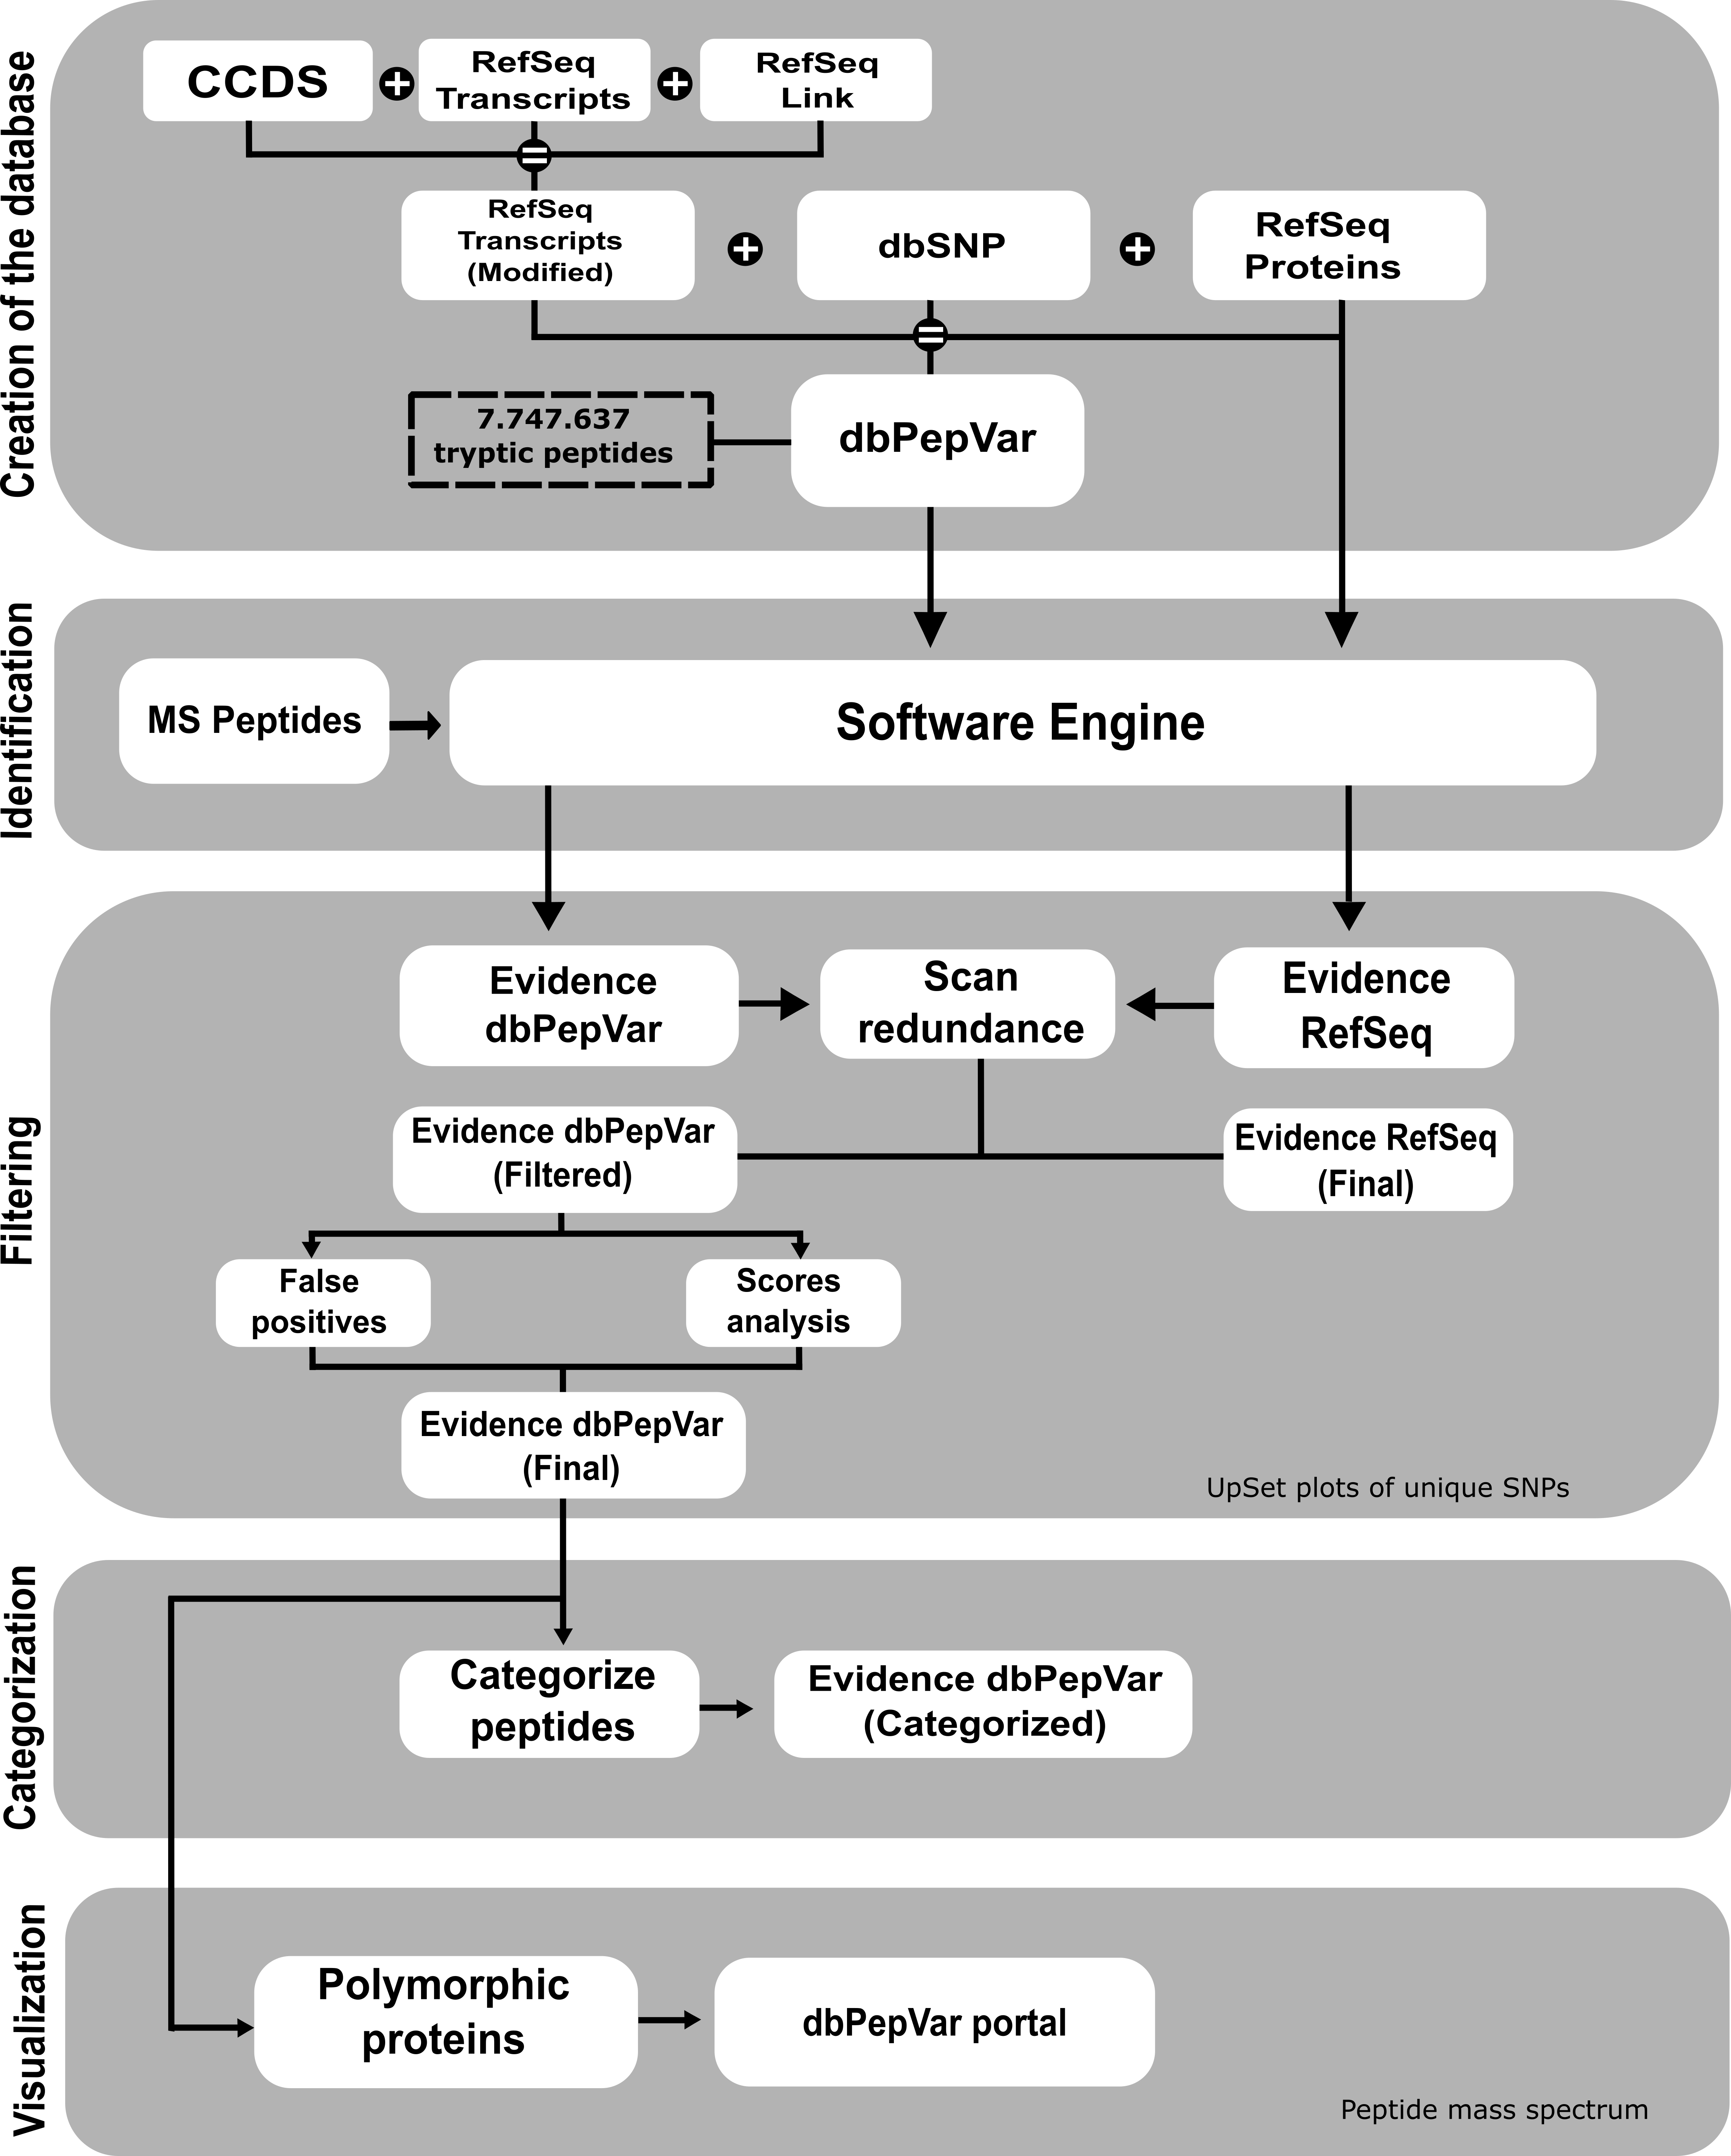
\includegraphics[width=0.8\linewidth]{fig1.png}
\caption{ 
\textbf{Workflow of dbPepVar creation and the analysis of the results. Database creation step}: The first step consists of generating a multi-fasta transcript file containing information about the position of the beginning of the reading frame, the transcript identifier, and the reference protein. This information was obtained from CCDS (Consensus Coding Sequence) and RefSeq Link files, which contain the association between CCDS identifiers, Refseq protein, and transcribed RefSeq. The modified transcript Refseq was used to generate the sequences with frameshift and stop-loss mutations. The dbPepVar integrates peptides information, types of mutations, and transcripts data from RefSeq proteins and dbSNP. \textbf{Peptide identification step}: The search process uses each base individually (dbPepVar and RefSeq) to identify the peptides.\textbf{Filtering step}: In this step, the identified peptides are checked in both bases (dbPepVar and RefSeq) and verified if they have the same MS spectrum. In a redundancy case, the variant peptide with a higher score was kept. The variant peptides with scores less than 50 and false positives were removed. The false positives are the variant peptides with enzymatic cleavage error whose position differs from the reference protein. \textbf{Classification step}: In this step, variant peptides are classified according to the type of mutation. \textbf{Visualization step}: In the last step, the evidence tables of each cancer analyzed are available at the portal dbPepVar, and the data is integrated with the mass spectra visualization tool, Proteogenomics Viewer.\label{fig1}}
\end{figure*}

%\Figure[t!](topskip=0pt, botskip=0pt, midskip=0pt){fig1.png}{\textbf{Workflow of dbPepVar creation and the analysis of the results. Database creation step}: The first step consists of generating a multi-fasta transcript file containing information about the position of the beginning of the reading frame, the transcript identifier, and the reference protein. This information was obtained from CCDS (Consensus Coding Sequence) and RefSeq Link files, which contain the association between CCDS identifiers, Refseq protein, and transcribed RefSeq. The modified transcript Refseq was used to generate the sequences with frameshift and stop-loss mutations. The dbPepVar integrates peptides information, types of mutations, and transcripts data from RefSeq proteins and dbSNP. \textbf{Peptide identification step}: The search process uses each base individually (dbPepVar and RefSeq) to identify the peptides.\textbf{ Filtering step}: In this step, the identified peptides are checked in both bases (dbPepVar and RefSeq) and verified if they have the same MS spectrum. In a redundancy case, the variant peptide with a higher score was kept. The variant peptides with scores less than 50 and false positives were removed. The false positives are the variant peptides with enzymatic cleavage error whose position differs from the reference protein. \textbf{Classification step}: In this step, variant peptides are classified according to the type of mutation. \textbf{Visualization step}: In the last step, the evidence tables of each cancer analyzed are available at the portal dbPepVar, and the data is integrated with the mass spectra visualization tool, Proteogenomics Viewer.\label{fig1}}

Peptide identifications were carried out using publicly available MS data, by performing MS/MS searches in each dbPepVar and Refseq databases separately. The results obtained were submitted to a filtration step that resulted in the data shown in Table S1. The table shows the number of unique peptides identified for the respective types of cancer and the search database used. A removal criterion based on identification scoring was rigorously applied to peptides derived from the dbPepVar database to guarantee the reliability of the identification. The identification of the variant peptide was only considered if: i) the MS spectrum was exclusively identified in the dbPepVar database; ii) the same spectrum providing conflicting identifications in each database, the dbPepVar result must have a score value higher than 20\% compared to the identification derived from Refseq. For example, the peptides sequences TEIQGIIGQIDEVSIEK (dbPepVar; NP\_004864.1) and AAAAVSESWPEIEIAER (Refseq; NP\_065761.1), were identified for the same MS spectrum (MS/MS Scan Number = 89008 and Raw File = 20131021\_EXQ3\_FaCo\_SA\_CL\_ME180\_B) in the ovary sample CL-ME180, with score values of 107.4 and 96.1, respectively. In this case, the reference peptide was kept and the variant peptide was deleted from the analysis. The adopted criterion provides an additional level of certainty in the identification of the variants present in the samples. A range of 220,405 to 341,906 variant identified peptides were found to have conflicting MS scans with reference sequences by cancer type. After analyzing the scores, 1,429 to 9,735 variant peptides remained. To remove experimental error introduced by the concatenation of variant peptides necessary to the database construction, peptides with missed tryptic cleavage sites and whose location differed on the reference proteins were regarded as false positives and excluded. Variant peptides found on the reference database were discarded as well. All identified peptides in RefSeq and dbPepVar and their MS identification features (score, mass, mass error, and others) are available on the portal by accessing the ``evidence tables'' tab.
When also considering peptide spectrum matches (PSMs) that were identified only in the dbPepVar search, the following number of variations were detected: 3,726 in the ovarian cancer samples, 2,543 in the prostate cancer samples, 2,661 in the breast cancer samples, and 2,411 in the colorectal cancer samples (Table S1). We estimated the number of peptides specific to the types of mutations used in the construction of dbPepVar to verify the proportion concerning the different types of cancer. As expected, most mutations identified are missense SNPs (Table \ref{tab1}), but there are also peptides with small in-frame indels (3-4\% avg), frameshift indels (\~1\% avg), and a few other characterized as UTR variation, stop-loss and c-terminal peptides derived from premature termination codons (average $<$ 0.5\%). 



\begin{table}
\caption{Number of unique peptides identified for the types of cancer: ovary (OvCa), prostate (PrCa), breast (BrCa), and colorectal (CrCa).}
\label{table}
\setlength{\tabcolsep}{3pt}
\begin{tabular}{|l|l|l|l|l|l|}
\hline
\textbf{Cancer Samples} & \textbf{SNP} &  \textbf{INDEL} & \textbf{Frameshift} &  \textbf{Stop Loss} & \textbf{UTR variation} \\ \hline
OvCa & 3.460 & 197 & 34 & 16 &  19\\
PrCa & 2.340 & 139 & 29 & 10 & 26 \\
BrCa & 2.501 & 117 & 20 & 6 & 18\\
CrCa & 2.266 & 104 & 22 & 8 & 11 \\
\hline
\end{tabular}
\label{tab1}
\end{table}

After classifying and counting the identified variants, those were organized as unique or shared between samples. This last step required the use of the SNP identifier (rs, reference sequence) as a unique key to each mutation. The shared and unique counts according to the SNP identifier can be seen in Fig. \ref{fig2}. Fig. \ref{fig2}a shows that ovarian cancer has most of the identified mutations with 3,684 SNPs (horizontal bar graph), of which 2,281 were unique to the sample (vertical bar graph). From all SNPs identified, there are 365 shared by all selected colorectal, prostate, breast, and ovarian samples, as shown by the connecting dots at the bottom of Fig. \ref{fig2}a (sixth bar from the left). Prostate and breast cancer samples share the highest number of common SNPs, with 437 entities. Prostate and colorectal cancer samples have the least, with 81 SNPs in common. There are 248 entities shared for three types of cancers: ovarian, prostate, and breast. The prostate samples have less exclusive SNPs, but share most SNPs with other cancers. A similar pattern arises among less frequent mutations ($<$ 5\%) (Fig. 2B). While through this type of analysis it is not possible to discriminate specific cancer mutations from those that were already present in the donors genomic background, comparing unique and shared SNPs in such samples might raise interesting hypotheses about the clinical condition under study.


\begin{figure*}[tp]%
\centering
%{\color{black!20}\rule{213pt}{37pt}}
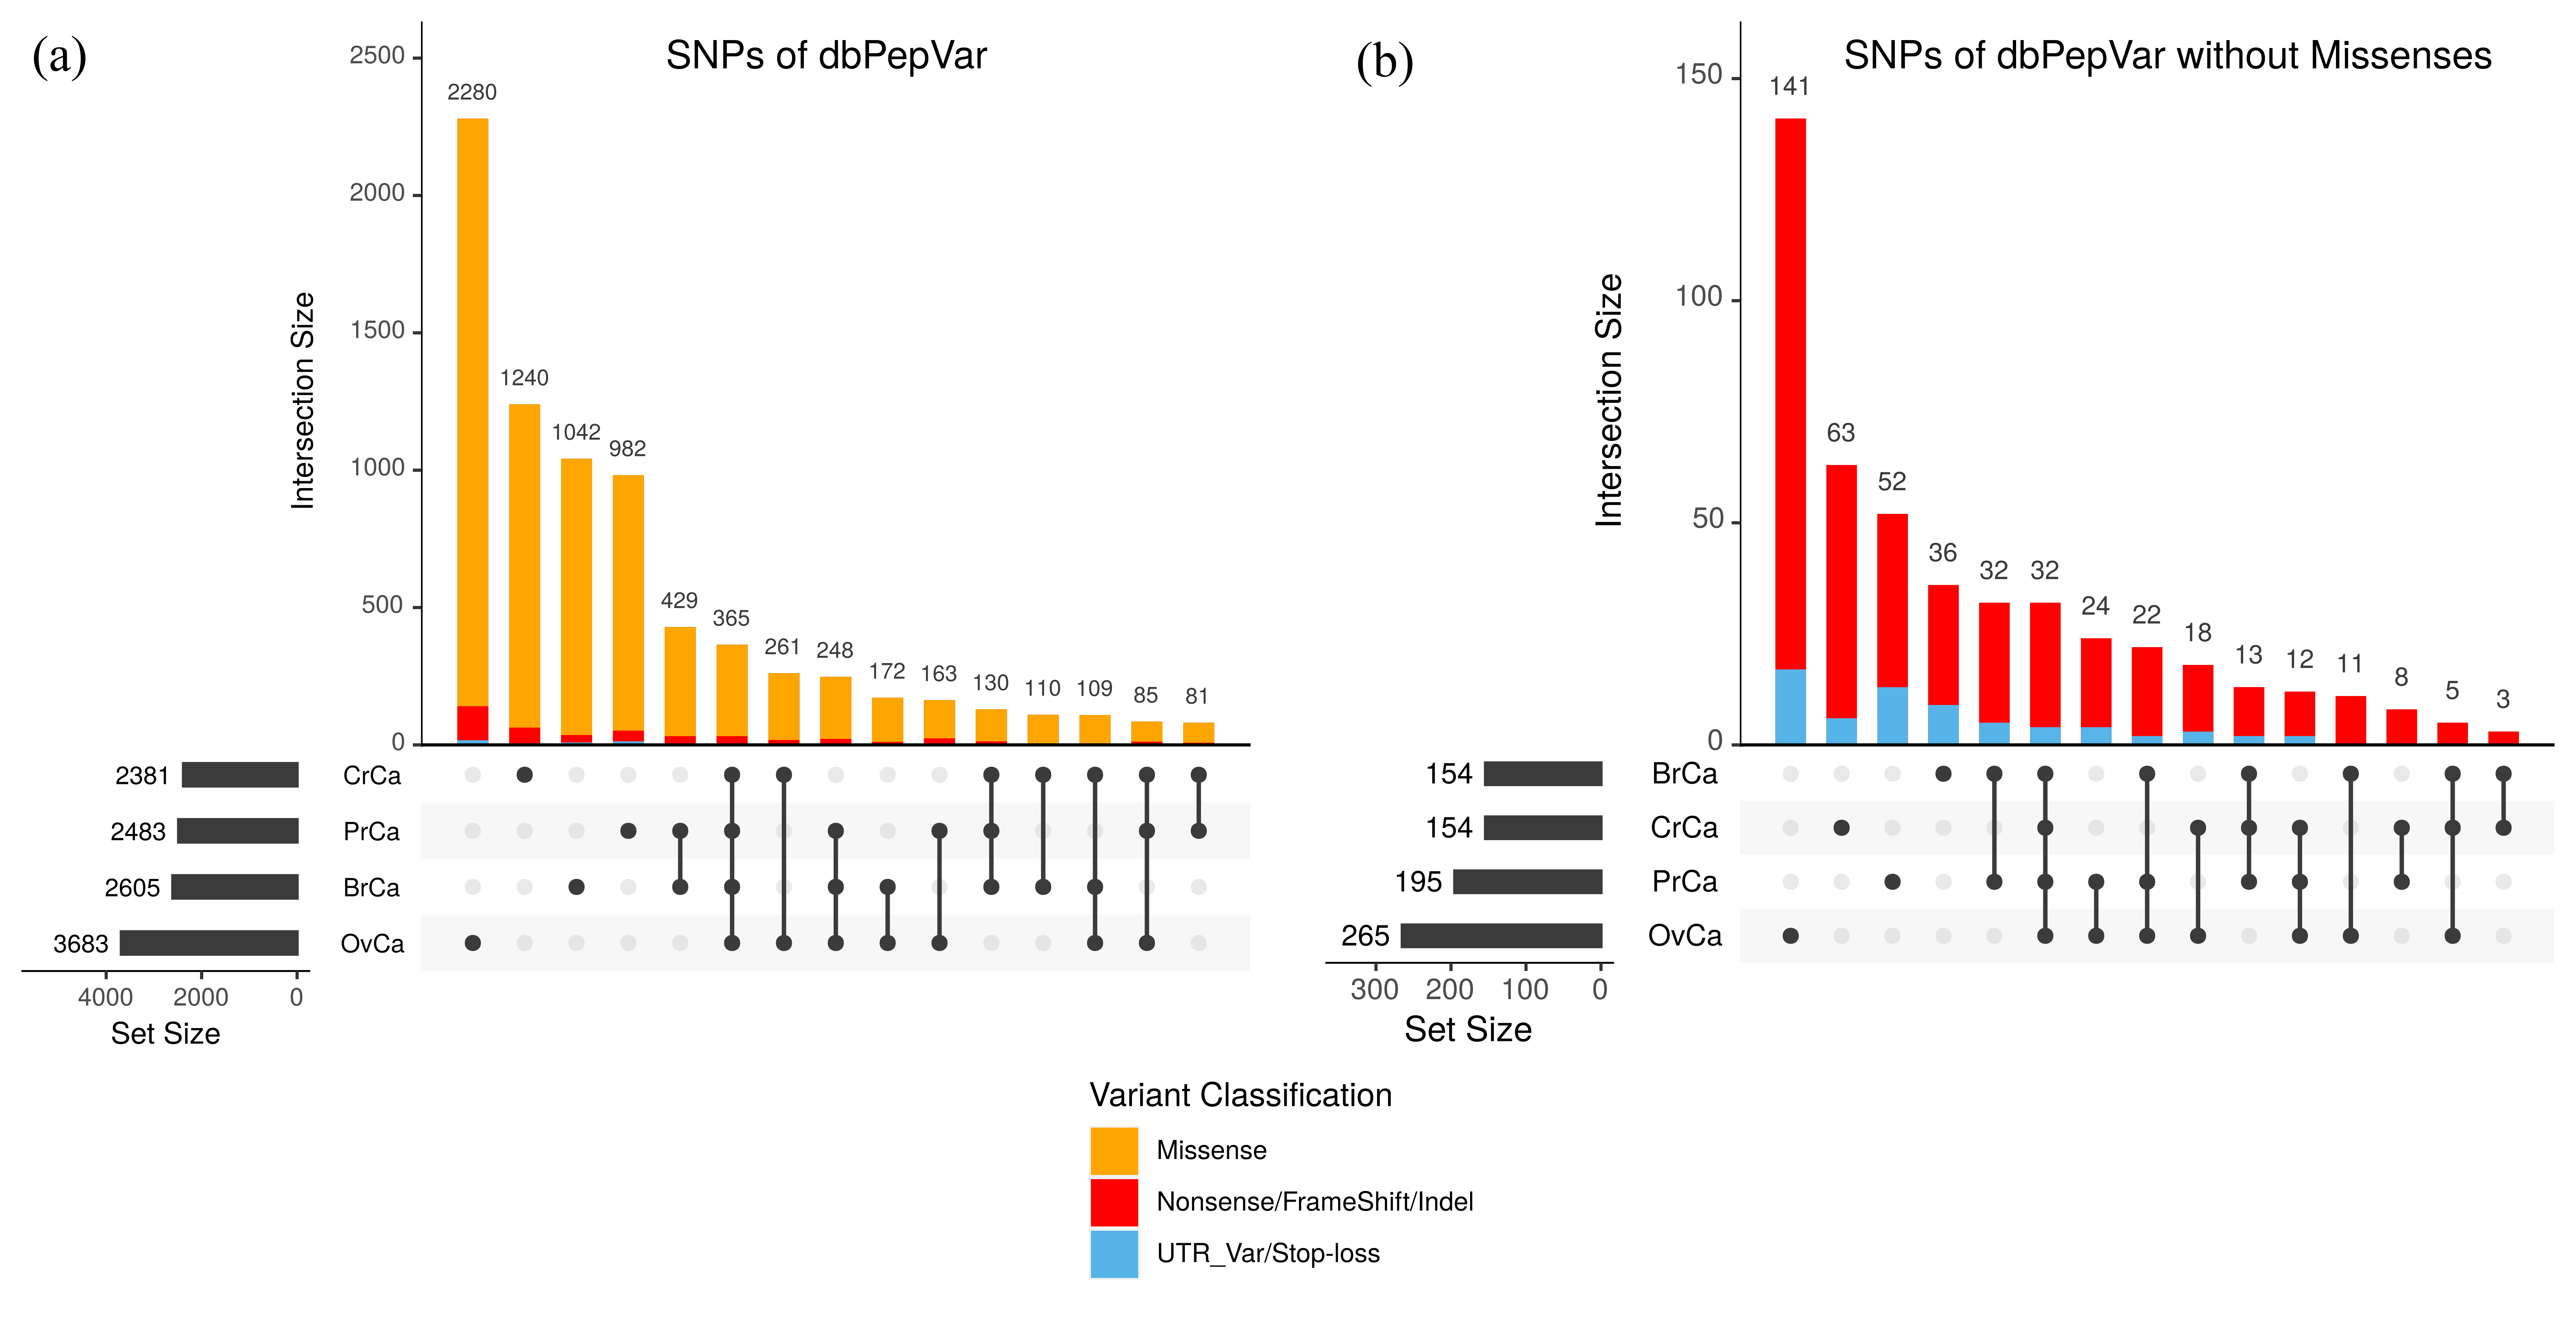
\includegraphics[width=1\linewidth]{fig2.png}
\caption{Variant distribution by sample typesand frequency of unique and shared variants from dbPepVar found in ovary (OvCa), prostate (PrCa), breast (BrCa) and colorectal (CrCa) cancer samples. The vertical bars show the number of identified variants for each sample combination, which is indicated by the vertical line and dots in the lower portion of the figure. (a) Data where missense mutations (orange) are considered. (b) Missense mutations are removed from the data, red bars indicate indel observations and blue bars indicate UTR and stop loss mutations. \label{fig2}}
\end{figure*}

%\Figure[t!](topskip=0pt, botskip=0pt, midskip=0pt){fig2.png}{Variant distribution by sample typesand frequency of unique and shared variants from dbPepVar found in ovary (OvCa), prostate (PrCa), breast (BrCa) and colorectal (CrCa) cancer samples. The vertical bars show the number of identified variants for each sample combination, which is indicated by the vertical line and dots in the lower portion of the figure. A) Data where missense mutations (orange) are considered. B) Missense mutations are removed from the data, red bars indicate indel observations and blue bars indicate UTR and stop loss mutations.   \label{fig2}}

\subsection{The web portal}

The data built into dbPepVar offers a wide range of potential opportunities for data mining and analysis. Our database, built using Shiny R, is available at \url{https://bioinfo.imd.ufrn.br/dbPepVar/}  and can be used by life science researchers who do not have command line experience. Here, we present a glimpse of the potential that dbPepVar has for the discovery of new data (Fig. \ref{fig3} and \ref{fig4}). However, this paper does not cover the full extent of the data or all potential applications of the platform, which is available as an open resource for the researcher to use in their investigations.

The first menu (``dbPepVar'') contains a summary of the data accessible through the portal (Fig. \ref{fig3}). The graphical displays were separated by section according to the type of data and analysis that can be performed. Broadly, the initial section reports the distribution of samples, peptide sequences, and unique polymorphisms filtered by cancer type or by variant type. The latter sections summarize different aspects of the database in graphical and table format. More specifically, dbPepVar users can view graphs of the distribution of peptides and SNPs by cancer type and mutation classification (SNPs graph only). In the second section, users can explore and visualize the count of the most mutated genes, segregated by cancer type and with a responsive table explicitly showing the displayed data. As with all graphs in the portal, Plotly tools (i.e. lasso or box select) are available and allow comparing data, filtering by cancer type and gene groups from a threshold that can be defined by counting SNPs identified per sample. The responsive table also allows to filter and visualize the number of samples that have a mutation in a specific gene according to the type of cancer. Similar analysis can be done with the graph and table provided in the following sections.

The third section of the first menu exhibits the number of SNPs per gene, which may be used to build a mutational panel for each cancer type and gene of interest. The fourth and fifth sections are dedicated to amino acid change counts by sample and by SNP, respectively. In this way, it is possible to observe, at the proteomic level, the most frequent amino acid exchanges for different cancers and SNPs, which may help understand which mutations propagate from the genome to the proteome. Two additional sections summarizing other layers of integrated information are then displayed, without tables: one with chemical property changes of amino acids sorted by cancer type, where `Multiple' refers to samples with frame-shift mutations, and another showing the distribution of mutated genes by chromosomal location. Thus, users can interactively perform two tasks: (i) filter and visualize the most frequent changes in amino acids according to cancer type, and (ii) filter and visualize the common exchanges between chemical groups of amino acids. 



\begin{figure*}[htpb]%
\centering
%{\color{black!20}\rule{213pt}{37pt}}
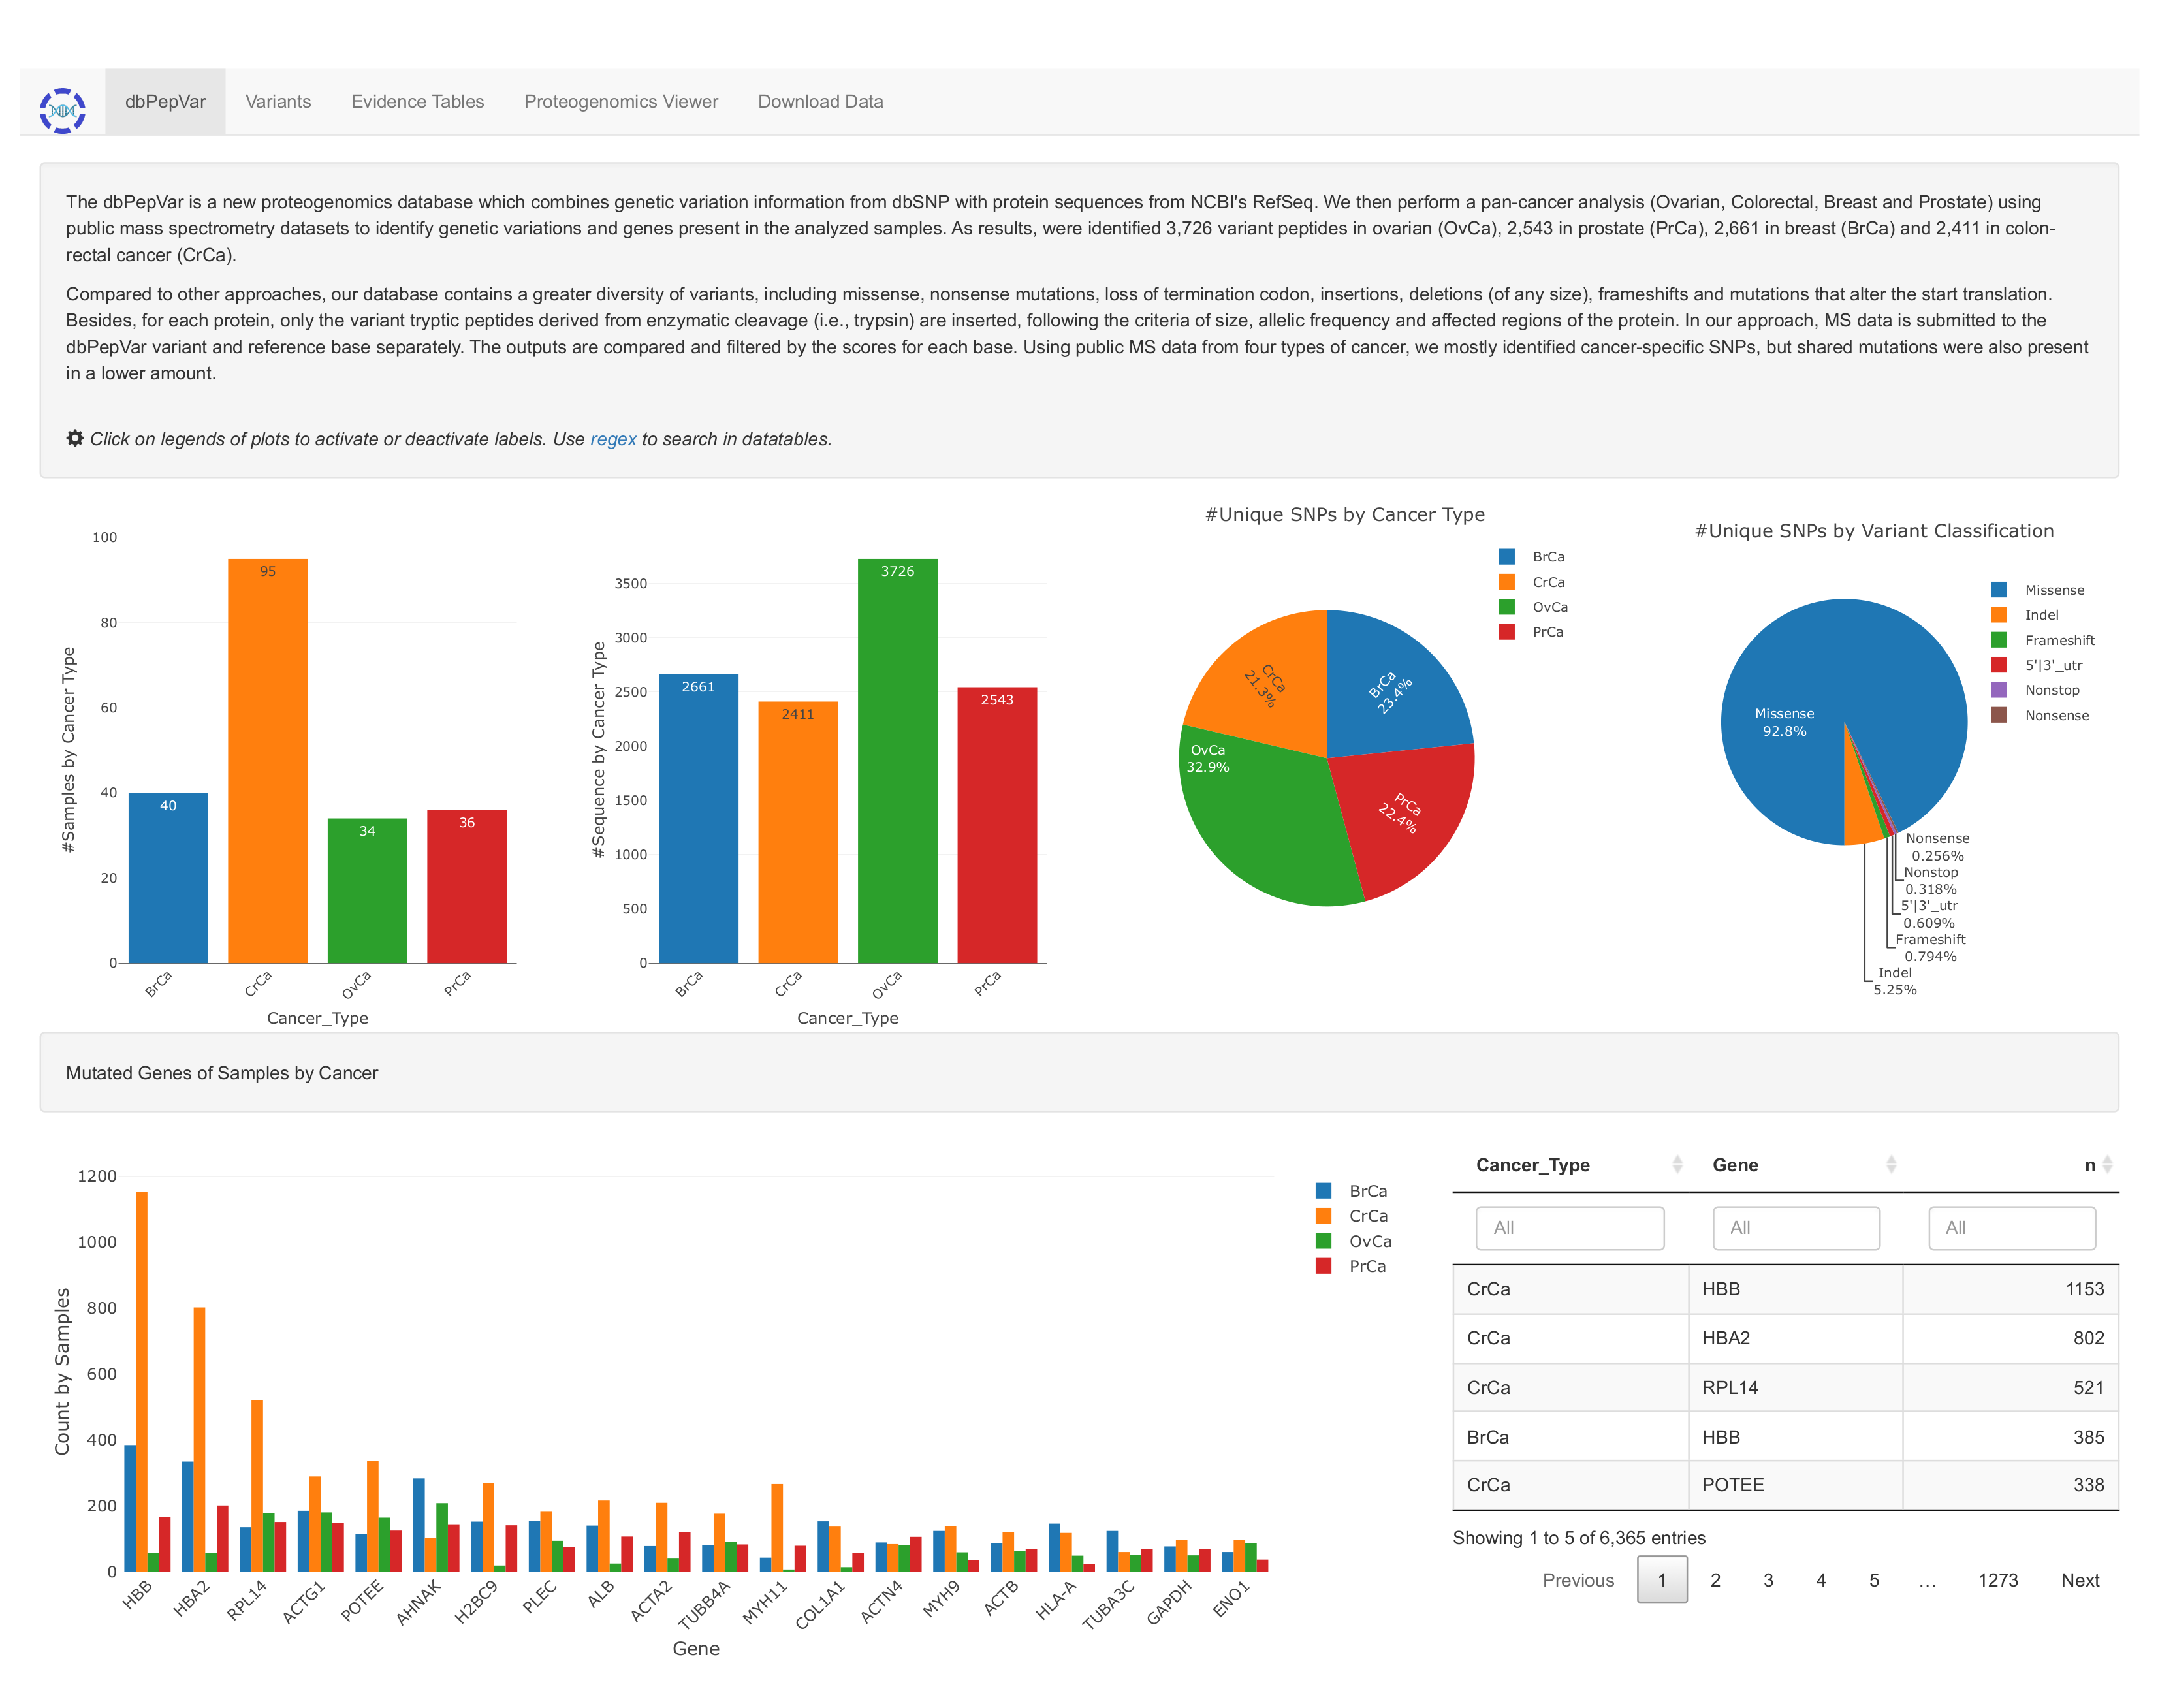
\includegraphics[width=1\linewidth]{fig3.pdf}
\caption{ 
The dbPepVar portal. Main Page - View of initial page containing the summary information of the samples, peptide sequences, and unique polymorphisms.  \label{fig3}}
\end{figure*}

%\Figure[t!](topskip=0pt, botskip=0pt, midskip=0pt){fig3.png}{The dbPepVar portal. Main Page - View of initial page containing the summary information of the samples, peptide sequences, and unique polymorphisms.  \label{fig3}}

The second menu (``Variants'') shows the actual dataset in an interactive format, where users can perform data mining and generate insights for their research (Fig. \ref{fig4}a). This action can be done by selecting all or single rows with up to 27 columns that describe each mutation. The table includes links to GeneCards, NCBI protein, and dbSNP. Users can filter on any of the provided columns using plain text and regular expressions. Recovered results can be downloaded as CSV or PDF formatted files (all pages or current page only). The third menu (``Evidence Tables'') is constructed by parsing the evidence files, which combine all information about the peptides identified by MS and is normally the only information needed for processing the results (Fig. \ref{fig4}b). It is from the evidence file that the other results presented on the portal are generated. Each type of cancer has an evidence file that can be accessed in its respective tab (BrCa, PrCa, OvCa, CrCa). Every file contains peptide information such as its amino acid sequence, post-translational modifications, the number of enzyme missed cleavages, its mass/charge ratio, identification scores, intensity, gene and  protein names where it belongs, and more. The displayed columns can be changed by selecting specific columns. By default, unique rows are displayed, but all rows may be selected. It is also possible to download filtered information in PDF or CSV format (all pages or current page only).


\begin{figure*}[htpb]%
\centering
%{\color{black!20}\rule{213pt}{37pt}}
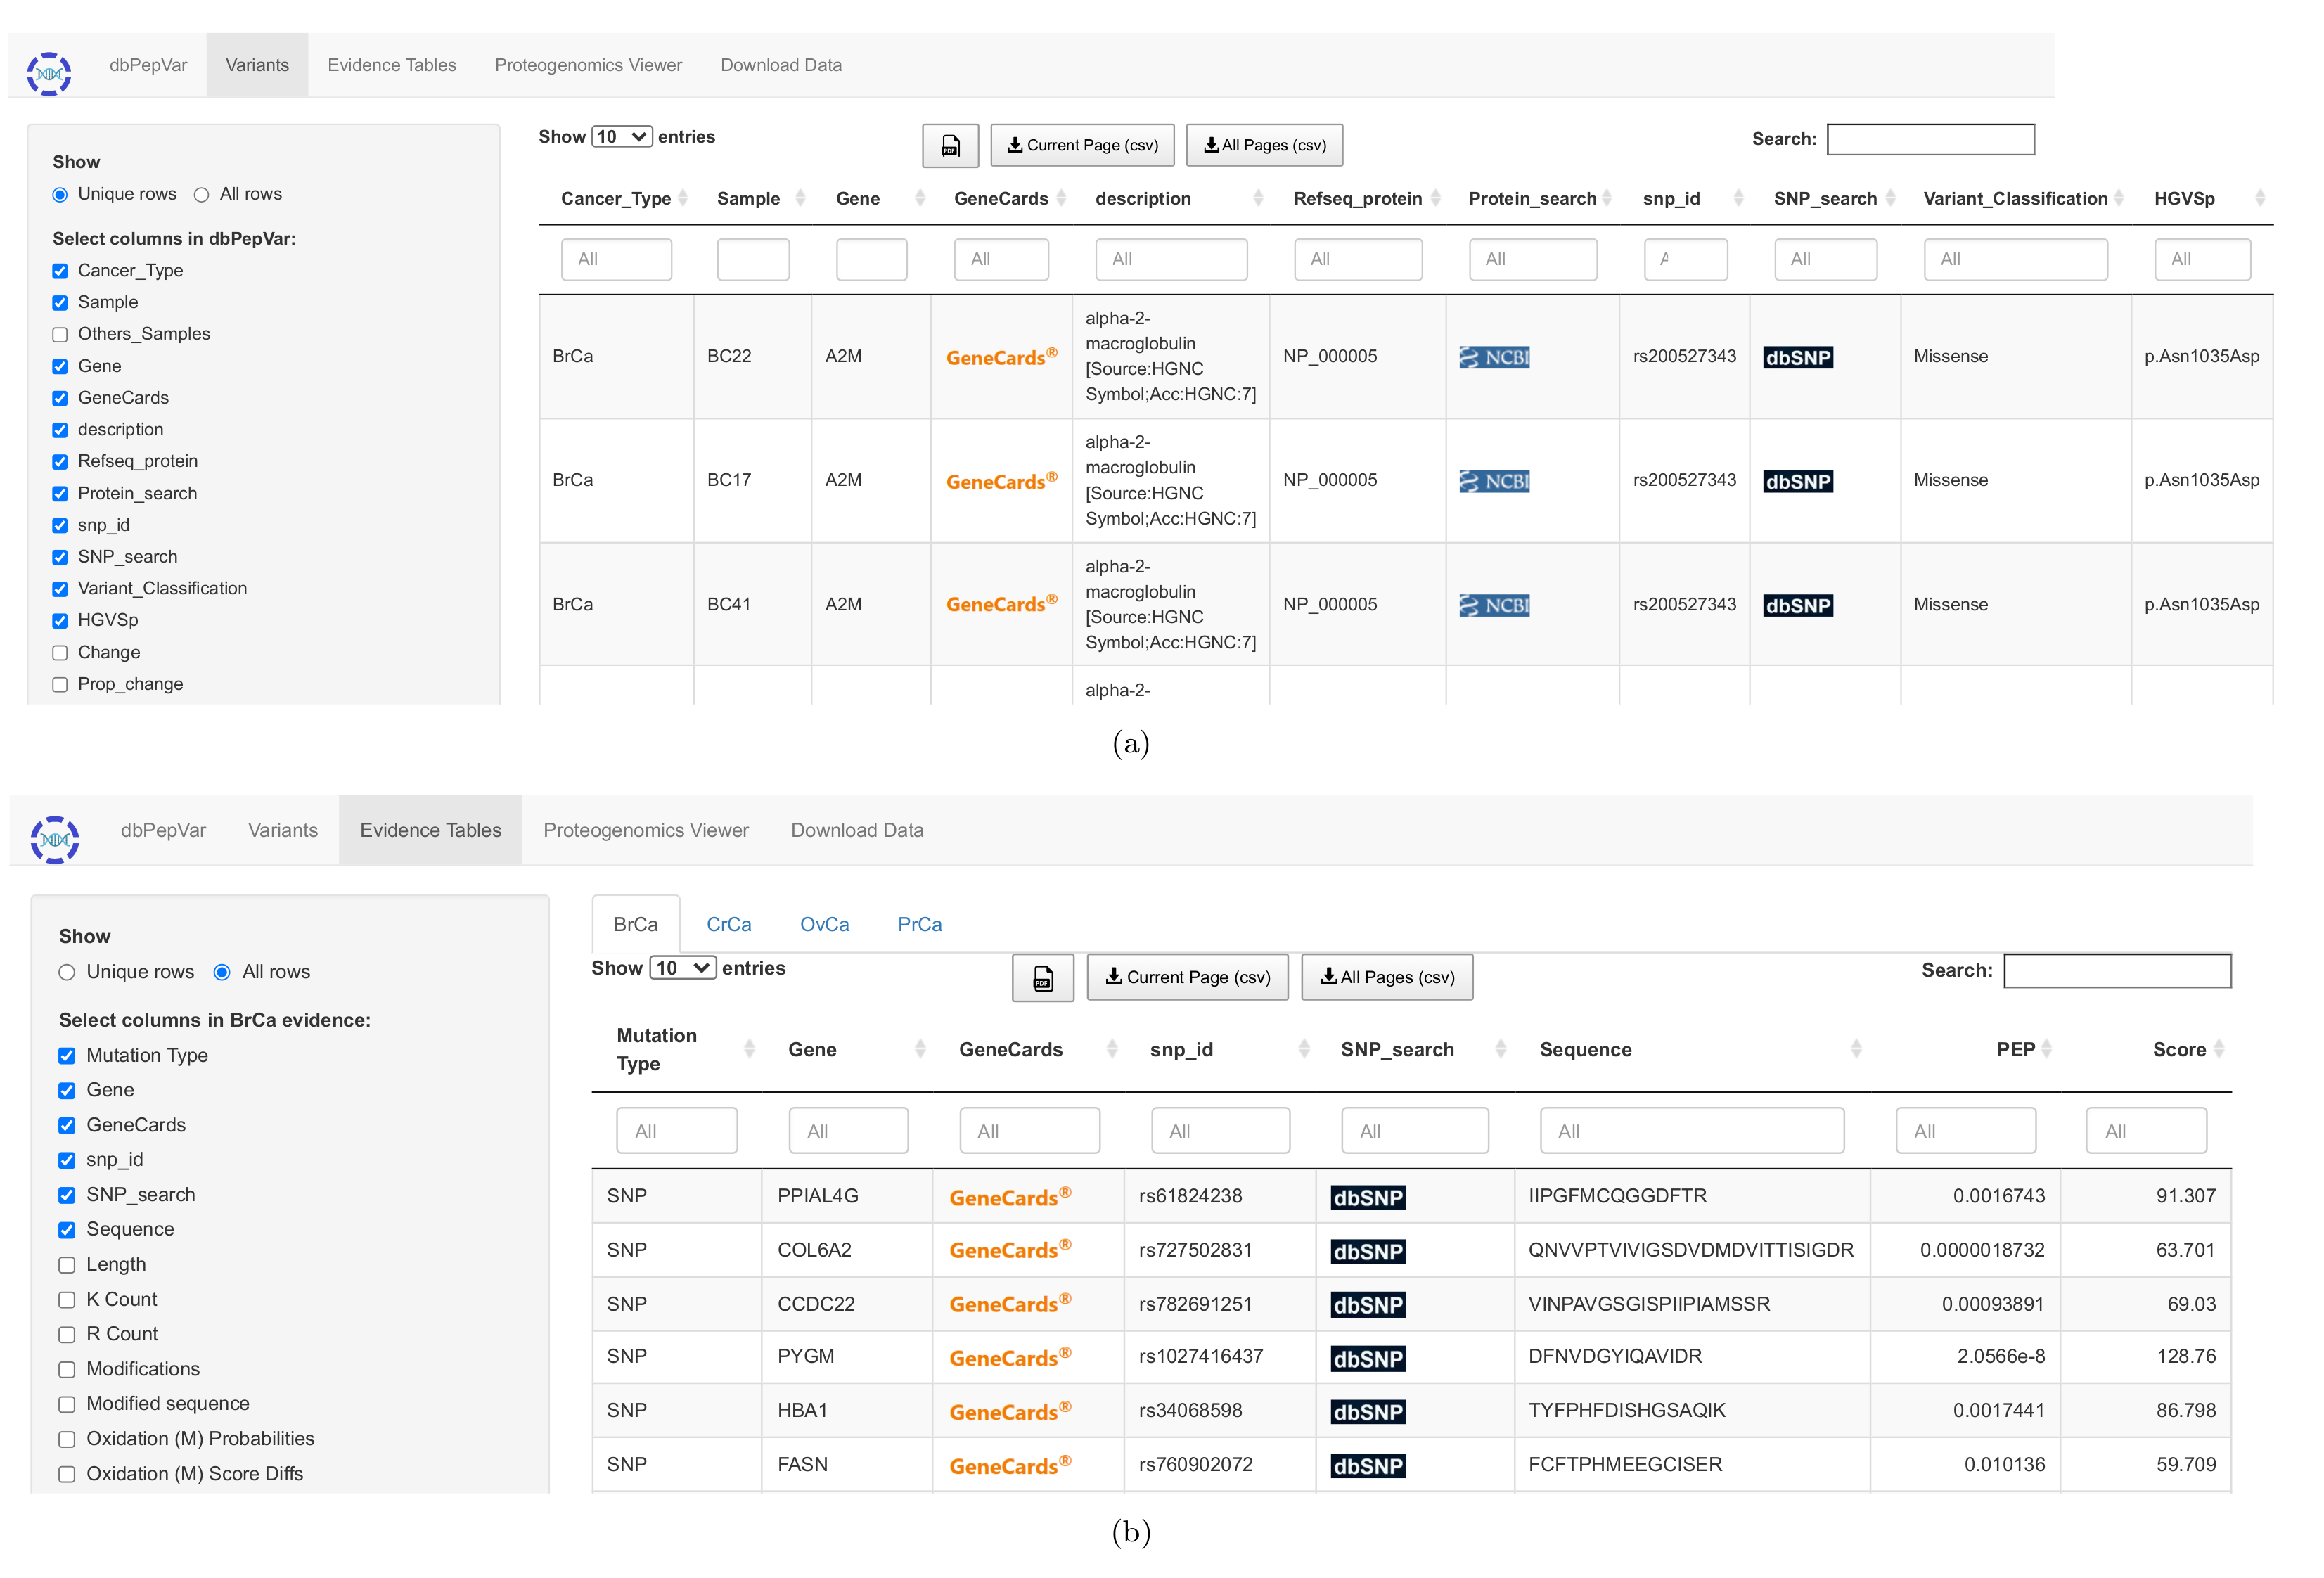
\includegraphics[width=1\linewidth]{fig4.pdf}
\caption{ 
Variant and Evidence menus. \textbf{(a)} The variant menu presents a table with 27 filterable columns to describe each mutation, 11 of which are shown by default. \textbf{(b)} The evidences menu has the actual data used to extract information available at dbPepVar. The parsed data is shown in tabulated  format and can be filtered by users through 75 columns, eight of which are presented by default.}\label{fig4}
\end{figure*}

%\Figure[!t](width=0.9\linewidth){fig4.png}{Variant and Evidence menus. A) The variant menu presents a table with 27 filterable columns to describe each mutation, 11 of which are shown by default. B) The evidences menu has the actual data used to extract information available at dbPepVar. The parsed data is shown in tabulated  format and can be filtered by users through 75 columns, eight of which are presented by default.\label{fig4}}


Next, the ``Proteogenomics Viewer'' menu \cite{Kroll2017-ab} integrates genomic and proteomic data, providing a genetic view of peptides in a sliding panel with their respective Peptide Spectrum and Peptide Expression. The search is performed by the name of the gene of interest and, after selecting it, the identified variant peptide sequences and its exonic location are shown. Finally, the ``Download data'' menu contains the files referring to the multi-fasta containing the mutated protein sequences and the log files containing information about SNPs identifiers, proteins, the position of the peptide in the protein, and mutated peptides and reference. It is also possible to obtain a detailed description of the information in each file and its respective construction process. 

Different proteogenomic approaches have developed web portals for data availability and analysis, using different criteria. Therefore, we listed the major databases for variant proteins and compared them with dbPepVar to highlight the unique features of our approach. The result of this comparison can be seen in Table \ref{tab2}. 


\begin{table*}
\caption{Comparison of dbPepVar with the characteristics of databases proposed by Literature.}
%\setlength{\tabcolsep}{3pt}
\begin{tabular}{|p{0.15\linewidth}|p{0.07\linewidth}|p{0.2\linewidth}|p{0.2\linewidth}|p{0.05\linewidth}|p{0.16\linewidth}|}
\hline
Databases & 
Separate peptide files & 
Mutation types & 
Chemically guided filtering & 
Online Database & 
Data sources 
\\ \hline
CanProVar  &
No  &
Missense, insertions, and deletions of single amino acid, frameshifts, stop-loss, splice-site  &
Not reported  &
Yes  &
COSMIC, HPI, TCGA, OMIM, BIOMART, Sjoblom et al.\cite{Sjoblom2006-gy}, Greenman et al. \cite{Greenman2007-jg}, Ding et al. \cite{Ding2008-fg}
\\ \hline
Swiss-CanSAAVs  &
No  &
Missense  &
Excluded Ile / Leu-Leu/Ile (post-processing), variant tryptic peptides with two missed cleavage sites.  &
Yes  &
UniProtKB/ Swiss-Prot, CanProVar, humsavar  
\\ \hline
dbSAP &
No &
Missense &
Peptide length ($>$~9~Aa), redundant sequence excluded. &
Yes &
Uniprot, PMD, HPMD, MSIPI, COSMIC, dbSNP, Ensembl, CanProVar
\\ \hline
Alfaro et al. [2017] &
Yes  &
Missense, insertions, deletions, frameshifts, stop-loss, and fusions. &
Peptide length ($>$6Aa), variant tryptic peptides with two missed cleavage sites, redundant sequence excluded (pre-processing) &
No &
Uniprot, COSMIC, dbSNP, Exome set, RNA set
\\ \hline
dbPepVar &
Yes &
Missense, UTR variation, stop-loss, frameshift, insertions, deletions. &
Peptide length ($>$~6~Aa and $<$36~Aa), redundant sequences excluded (post-processing), fully tryptic variant peptides, in silico cleavage of the initial methionine into peptides with two or more mutations, combinatorial analysis of mutations in peptides with more than one variant. &
Yes &
dbSNP, RefSeq/NCBI\\
\hline
\end{tabular}
\label{tab2}
\end{table*}

In recent years, many new biological databases of mutant proteins have been developed and published. However, all published databases have distinct and particular scopes, and to our knowledge, no databases have been published reporting the variants for cancer proteogenomics data using our reverse engineering methodology, i.e. identifying genetic mutations from altered proteins. In particular, the dbPepVar uses more refined criteria to detect peptides that accurately represent the actual peptide, such as changes in cleavage sites, peptide size, and peptides with combined mutations.

\section{DISCUSSION}
    
The characterization of genetic mutations in their protein products is a key step to understanding their role in diseases such as cancer. However, MS-based approaches do not routinely allow the identification of polymorphisms in samples of interest. In this study, a database of variant peptides (dbPepVar) to be used in proteomics was created combining information of proteins from dbSNP and RefSeq. The dbPepVar identified genetic changes at the protein level in MS samples from four different types of cancer. In proteomics, the identification of genetic variants depends on the presence of such variants in the database used during MS spectrum matches. Many publications had suggested diverse approaches to improve such identification coverage. This includes adding variant tryptic peptides concatenated to the reference sequence entry, such as observed in CanProVar \cite{Li2010-px,Zhang2017-yz}, Swiss-CanSAAVs \cite{Song2014-bn} and dbSAP \cite{Song2014-bn,Cao2017-pv}, which may lead to false-positive identifications. Adding variant and reference peptides to the same fasta file can increase the probability of matching an inappropriate, but high-scoring peptide among the large number of available sequences. For instance, a variant peptide may be correctly assigned to an isobaric reference peptide, according to the spectrum, but still correspond to a different reference protein. Also, a peptide variant can be mismatched to a spectrum because the change in mass caused by a mutation coincides with the change in mass associated with a post-translational change in a different peptide. In dbPepVar, the variant peptides are incorporated in a single fasta file and the search is performed separately, allowing to distinguish between mutated and reference peptides during the identification process. In addition, a set of filters based on MS scores, removal of redundant sequences, and analysis of cleavage errors were developed to ensure that the identified peptides match the reported protein. The database built by Alfaro and coworkers \cite{Alfaro2017-vp} presents a similar approach. However, they only consider the minimum size of the peptide incorporated in its variant base (7 residues); dbSAP also considers only the minimum size of the peptide (10 residues). Mass spectrometry-based proteomics has some limitations, including the difficulty of identifying peptides that have very small or large sizes. For the peptides to be identified with greater precision, they must have a size in the range of 7-35 amino acid residues \cite{Swaney2010-px}. To avoid losing the identification of variants, dbPepVar also considered this interval as a parameter to determine the number of amino acid residues of the peptides present in the base. Swiss-CanSAAVs and the database proposed by Alfaro and coworkers have peptides with two missing cleavage sites, while dbPepVar has only fully tryptic peptides. Including peptides with missing cleavages in protein quantification does not produce significant differences in precision, accuracy, specificity, and sensitivity compared to the use of fully tryptic peptides \cite{Chiva2014-jo}. 

 The dbPepVar also performs the N-terminal methionine processing for peptides that have two or more mutations, as the sequences are generated by the concatenation of the peptides. This process is done to ensure the identification of variant peptides from proteins where the N-terminal methionine has been cleaved by co-translation by the enzyme methionine aminopeptidase \cite{Wingfield2017-he}. The approaches presented in Table \ref{tab2} assume that all digested peptides cannot have more than a single mutation. These features reduce search time, avoiding the exhaustive search for all possibilities, but naturally prevent coverage of all possible variant peptides at the same time \cite{Seunghyuk_Choi2020-es}. A key advantage of dbPepVar lies in its ability to identify multiple combinatorial variants, considering all possible mutations contained in the same peptide. To avoid increasing the search space, combinations were made only for mutations with an allelic frequency greater than 5\%. It is known that non-random genetic variations of a haplotype tend to occur together \cite{CHOONG2020}. Therefore, the discovery of peptides with multiple mutations can be interpreted as a disease-associated haplotype, because the altered phenotypes often result from a combination of multiple factors \cite{Na2012-qm}. For instance, peptides with multiple variations have been reported in ovarian and lung cancer samples \cite{Woo2014-tk, CHOONG2020}.
 
dbPepVar was also customized to add mutation types that affect coding regions, such as SNPs, indels, variation of the translation initiation codon, and stop-loss. SwissCanSAAVs and dbSAP have only missense mutations; CanProVar and the database developed by Alfaro et al. have almost the same types of mutations incorporated as dbPepVar, except for gene fusion (Alfaro et al.) and splice site (CanProVar) mutations. The dbPepVar differs from these approaches by the addition of the UTR-variation/start codon variation mutations. This type of mutation affects the initial methionine, generating changes in the translation start and the untranslated region of the protein \cite{Parsons2015-by}. Thus, in the approach proposed by dbPepVar, the peptides were generated from the search for a new alternative translation start methionine. Clinical genetic testing has identified two variants related to endometrial and breast cancers likely to affect native translational initiation on the MLH1 and BRCA2 genes \cite{Parsons2015-by}. Although few peptides generated by this type of mutation have been identified, this finding highlights the existence of isoforms that are being expressed by the cell in diverse cancerous environments.

Another advantage of dbPepVar is the possibility of an association between mutations identified in cancer and genetic variations in populations, which can be made from information available in public databases, such as the TCGA. In this way, this information can be used to investigate the predisposition of individuals to the disease and how this variation propagates over generations. This data expands the scope of investigation of an individual's predisposition to cancer development, given their genetic makeup. Recently, a study was conducted showing that the genotypes of patients with congenital heart disease may be responsible for the increased risk of cancer \cite{Morton2021-ch}. Thus, the recognition that genotypes influence cancer risk can promote early clinical care and interventions and further promote lifelong health in patients.

The dbPepVar portal contains all the information presented in this work but is not limited to these findings. Each researcher can use it according to their research needs. The results described can be found by navigating to the ``variants'' tab and selecting the fields referring to the type of search intended. The direct link with dbSNP makes it possible to verify (i) whether the mutation identified in dbPepVar is associated with other congenital or acquired diseases throughout life and (ii) the frequency of a specific variant in different populations. dbPepVar's variant menu also has a field indicating the remaining percentage of the protein sequence due to amino acid loss in a protein with a premature termination codon (PTC). For example, by selecting the field ``PTC gene'' and filtering by ``TRUE'', it is possible to obtain the variant peptide sequences that cause protein shortening, as well as information associated with the quality of identification by MS and the relationship with other databases such as GeneCards, NCBI and dbSNP. Thus, this information may be useful in investigating the impact of the mutation concerning the reduction of the protein's polypeptide chain and its relationship with some disease or alteration of its biological function. CanProVar and dbSAP present a portal with some similar characteristics to dbPepVar. CanProVar has the option to visualize the alteration of KEGG biological pathways in cancer and links that direct the user to information on genetic ontology and protein-protein interaction networks. Swiss-CanSAAVs presents in its article a link that directs to the portal, but it is inactive. dbSAP has an exclusive tab for viewing post-translational modifications and another for viewing variant and reference peptide sequences according to tissue type or cell lineage. In dbPepVar, it is also possible to visualize the PTM through the evidence tables resulting from the identification by MS. These tables also served as input for the construction of theoretical protein sequences used to visualize the information presented in the Proteogenomics Viewer. Integrating this platform to dbPepVar is unique to our approach, so the user will access the expression of the peptides and their respective mass spectra, besides being able to visualize their exonic location in the genome.

dbPepVar presents a proteomics overview for several samples from different types of cancer, allowing researchers to search for information on the set of mutations that affect specific groups of samples, analyze the most frequent mutations and changes in amino acid residues, and have direct access to information regarding each type of mutation. Approaches based on mass spectrometry gain their limitations of the technique, for example, the absence of the mutant peptide in the identification due to size. In that case, the mutant tryptic peptide may be relatively small (e.g., less than six amino acids) and therefore difficult to reliably match the corresponding MS/MS spectrum.  

\section{CONCLUSION}

This work presents a new proteogenomic approach for building a database of variant peptides that helps identify genetic protein variations with mass spectrometry. The dbPepVar reports missense, nonsense, frameshift, indel, stop loss, and UTR variation mutations absent in major protein databases such as RefSeq/NCBI and UNIPROT. Furthermore, the peptides available in dbPepVar were obtained upon careful consideration of the number of amino acids in the sequence, alterations in cleavage sites, and post-translational modifications, which are essential biological characteristics for the reliability of the identification. We have also developed a web portal for the database in which provide information on samples of four cancer types: ovarian, colon-rectal, breast, and prostate. Our portal has different filters that help the user search for information on the genetic variations identified for each type of cancer. We also integrate our data into a platform to visualize mass spectrometry‐based peptide data and the corresponding genome alignments.

In the future, we aim to expand our database by adding other types of mutations and integrating them with other databases of genetic variations. Forthcoming research may investigate the relationship of the variants reported to the different types of cancer.

\section{The dbPepVar web portal}

The web portal was implemented with the R package `shiny' (v1.6.0). The packages required are `tidyverse' (v1.3.1) for data preprocessing, `vroom' (v1.5.5) for efficient reading data, `plotly' (v4.9.4.1) for interactive visualizations, and the `DT' (v0.19) for building interactive tables.

\section{Data Availability}

Publicly available datasets were analyzed in this study. 
Code used for analyses and to produce the figures is publicly available at: \url{https://github.com/terrematte/dbPepVar_codes}. 

\section{Abbreviations}

dbPepVar: new proteogenomics database; MS: Mass spectrometry; OvCa: ovary cancer of dbPepVar; PrCa: prostate cancer of dbPepVar; BrCa: breast cancer of dbPepVar; CrCa: colorectal cancer of dbPepVar; TCGA: The Cancer Genome Atlas; 

\section{Author Contributions}

LMC: conceptualization. LMC, PT: code implementations. LMC, VLS, JEK, PT: methodology. LMC, PT, TSF: composition and draft preparation. LMC, TSF, PT, GAS: composition, reviewing, and editing. GAS, SJS: supervision, funding, and infrastructure. All authors contributed to the article and approved the submitted version.

\section{Funding}

This work was supported by grants 23038.004629/2014-19 to GAS from the Coordenação de Aperfeiçoamento de Pessoal do Ensino Superior. GAS was also supported by grants 406630/2016-0 and 304422/2017-7 from Conselho Nacional de Desenvolvimento Científico e Tecnológico (CNPq). LMC, VLS, JEK, TSF were funded by CAPES –  Coordination for the Improvement of Higher Education Personnel formation programs.  This publication was supported by the Fund of the Federal University of Rio Grande do Norte.

\section{Conflict of Interest}

The authors declare that the research was conducted in the absence of any commercial or financial relationships that could be construed as a potential conflict of interest.

\section*{Acknowledgment}

The data processing was conducted with computational resources of the High-Performance Computing Center (NPAD) (\url{http://npad.ufrn.br}) and the Bioinformatics Multidisciplinary Environment (BioME) at UFRN (\url{https://bioinfo.imd.ufrn.br}).

%\appendices

%Appendixes, if needed, appear before the acknowledgment.


% The preferred spelling of the word ``acknowledgment'' in American English is 
% without an ``e'' after the ``g.'' Use the singular heading even if you have 
% m any acknowledgments. Avoid expressions such as ``One of us (S.B.A.) would 
% like to thank $\ldots$ .'' Instead, write ``F. A. Author thanks $\ldots$ .'' In most 
% cases, sponsor and financial support acknowledgments are placed in the 
% unnumbered footnote on the first page, not here.

%\bibliographystyle{plain}
%\bibliographystyle{unsrtnat}
\bibliographystyle{IEEEtranDOI}
\bibliography{references}


\begin{IEEEbiography}[{\includegraphics[width=1in,height=1.25in,clip,keepaspectratio]{author_lucas.jpeg}}]{Lucas Marques da Cunha}

received the B.S degree in Information Systems from University Center of Patos (UNIFIP), Paraíba, Brazil and the M.S degree in computer science from Federal University of Paraiba, Paraíba (UFPB), Brazil, in 2016. He is currently pursuing the Ph.D. degree in bioinformatics at the Federal University of Rio Grande do Norte (UFRN), Brazil and working as an Assistant Professor with the Faculty of Computer Science, Federal University of Rondônia (UNIR), Porto Velho, Rondônia. He is an expert on biologicals database development and forensic analysis on digital images. He developed a method for detecting tampering in digital images for different compression ratios.

He worked in remote learning at the Federal University of Paraíba and supervised several researches on technologies applied to education. He works with teaching programming for mobile devices for android using the Java language. He has over 6 years of research and teaching experience. His research interests include Artificial Intelligence, Explainable Machine Learning, Bioinformatics. Proteogenomics and Computational Modeling.
\end{IEEEbiography}

\begin{IEEEbiography}[{\includegraphics[width=1in,height=2in,clip,keepaspectratio]{author_patrick.png}}]{Patrick Terrematte} received a B.S. in systems analysis from Federal Institute of Education, Science and Technology of Rio Grande do Norte (IFRN), Rio Grande do Norte, Brazil, in 2011, and a M.S. degree in systems and computation from Federal University of Rio Grande do Norte (UFRN), Rio Grande do Norte, Brazil, in 2013. He has a Ph.D. in bioinformatics from UFRN at Bioinformatics Multidisciplinary Environment (BioME), Rio Grande do Norte, Brazil, in 2022. Currently, he is assistant professor at UFRN, Metropolis Digital Institute (IMD) in Brazil.

From 2016 to 2022, he was an assistant professor of Computing Engineering at Federal Rural University of Semi-arid, Department of Engineering and Technology (DETEC) in Brazil. He has published on survival prediction for clear cell renal cell carcinoma. His research interests include artificial intelligence, explainable machine learning, information theory, feature selection, bioinformatics, survival analysis, systems biology, computational modeling, and logic.
\end{IEEEbiography}

\begin{IEEEbiography}[{\includegraphics[width=1in,height=1.25in,clip,keepaspectratio]{author_tayna.png}}]{TAYNA DA SILVA FIUZA} received a B.S. degree in biotechnology from the Federal University of Ceara (UFC), Ceará, Brazil, in 2017, and a M.S. degree in bioinformatics from the Federal University of Rio Grande do Norte (UFRN), Rio Grande do Norte, Brazil, in 2019. She is currently pursuing a Ph.D. degree in bioinformatics at the Federal University of Rio Grande do Norte, Brazil.

She has worked with isolating proteins and carbohydrates from marine algae, evaluating their biological activities in animal models, animal cell culture and transfection. Today, her research interest includes the development of computational approaches for the identification of potential vaccine candidates in the genomes of pathogenic microorganisms and applying immunoinformatics tools for neglected diseases. 

\end{IEEEbiography}

\begin{IEEEbiography}[{\includegraphics[width=1in,height=1.25in,clip,keepaspectratio]{author_vandeclecio}}]{Vandeclécio Lira da Silva} 
received the B.S degree in computer science from the State University of Rio Grande do Norte (UERN), Rio Grande do Norte, Brazil, M.S degree in genetics from the Federal University of Pará (UFPA), Pará, Brazil and a Ph.D. in bioinformatics from the Federal University of Rio Grande do Norte (UFRN), Rio Grande do Norte, Brazil. He is currently a Postdoctoral Researcher at the Beneficência Portuguesa Hospital, in Sao Paulo, Brazil. 

He was a Bioinformatics Specialist at Duna Bioinformatics (2019-2020) and a Post Doctoral Researcher at the Laboratory of Human Genetic Diversity (LDGH) at Federal University Minas Gerais (2020-2022). He has experience in Computer Science, focusing on databases. His research interests include: piRNAs, gastric tissues, microarray and drosha. He has experience with cloud computing and AWS. 
\end{IEEEbiography}

\begin{IEEEbiography}[{\includegraphics[width=1in,height=1.25in,clip,keepaspectratio]{author_eduardo.jpg}}]{José Eduardo Kroll} 

received B.S. degree in pharmacy from the University of Mogi das Cruzes, Sao Paulo, Brazil, in 2006, an M.S degree in biotechnology from the same university and a Ph.D. in bioinformatics from the Federal University of Sao Paulo, Sao Paulo, Brazil. He currently works as a Bioinformatics Specialist at a hospital \& health care company (DASA), in Sao Paulo, Brazil.

He was a Senior Bioinformatician at the Institute for the Heart (2020-2021), a Chief Technology Officer at Duna Bioinformatics (2019-2020) and a Post Doctoral Researcher at the Brain Institute (2014-2018). His research interests include diagnostics, genomic profiling for disease risk, proteogenomics and cancer bioinformatics.

\end{IEEEbiography}


\begin{IEEEbiography}[{\includegraphics[width=1in,height=1.25in,clip,keepaspectratio]{author_sandro.jpg}}]{Sandro José de Souza} holds a degree in Biology from the Federal University of Parana, Parana, Brazil (1989) and a PhD in Biochemistry from the University of Sao Paulo, Sao Paulo, Brazil (1993). 

From 1995 to 1998, he was a Pew Latin American Fellow at Harvard University. He was one of the pioneers of genomics and bioinformatics in Brazil. He was an associate member of the Ludwig Institute for Cancer Research from 1999 to 2012. He is currently a Full Professor at the Brain Institute at UFRN. Elected by the World Economic Forum as a Young Global Leader in 2009. He was Tinker Visiting Professor at the University of Chicago in 2011. He is researcher 1A at Brazilian National Council for Scientific and Technological Development (CNPq).
\end{IEEEbiography}

%Possui graduação em Biologia pela Universidade Federal do Paraná (1989) e doutorado em Bioquímica pela Universidade de São Paulo (1993). De 1995 a 1998, foi Pew Latin American Fellow na Universidade de Harvard. Foi um dos pioneiros da genômica e da Bioinformática no Brasil. Foi membro associado do Instituto Ludwig de Pesquisa sobre o Câncer de 1999 a 2012. Atualmente é Professor Titular do Instituto do Cérebro da UFRN. Eleito pelo Fórum Econômico Mundial como um ?Young Global Leader? em 2009. Foi Tinker Visiting Professor na Universidade de Chicago em 2011. (Fonte: Currículo Lattes) 


\begin{IEEEbiography}[{\includegraphics[width=1in,height=1.25in,clip,keepaspectratio]{author_gustavo.jpg}}]{Gustavo Antonio de Souza} received the B.S. degree in biology from the Federal University of Parana, Parana, Brazil, in 1999, and the M.S and PhD degrees in molecular and cell biology from the University of Sao Paulo, Sao Paulo, Brazil, in 2004. He is currently affiliated to the Dept. of Biochemistry from Federal University of Rio Grande do Norte, Rio Grande do Norte, Brazil.

From 2005 to 2007, he was a Postdoctorate collaborator at the Max-Planck-Institut für Biochemie, Munich, Germany and from 2010 to 2017 he worked at the University of Oslo, Oslo, Norway. His research interests include developing computational approaches for the analysis of proteomic data for the identification of potential vaccine candidates in the genomes of pathogenic microorganisms.
\end{IEEEbiography}





\EOD

\end{document}
